\documentclass{template/socthesis}

\usepackage{subcaption} 
\usepackage{amsmath} 
\usepackage{enumitem} 
\usepackage{hyperref} % reference
\usepackage{gensymb} % balíček symbolů
\usepackage{booktabs}

\usepackage[toc,page]{appendix}
\usepackage{color} % balíček pro obarvování textů
\usepackage{xcolor}  % zapne možnost používání barev, mj. pro \definecolor
\definecolor{mygreen}{RGB}{0,150,0} % nastavení barev odkazů 
\usepackage{listings} % balíček pro formátování zdrojových kódů 
\usepackage[author=,status=final]{fixme} % vkládání poznámek  
% dva módy (status): draft (poznámky se zobrazují v PDF) / final (poznámky se nezobrazují v PDF)
\usepackage{multirow}
\usepackage{hyperref} % pro vkládání odkazu

\lstset { %
    language=C++,
    backgroundcolor=\color{black!5}, % set backgroundcolor
    basicstyle=\footnotesize,% basic font setting
}

\addbibresource{text.bib} % soubor s bibliografií
\nocite{*}

\titlecz{Postav si svého druhého robota} % český název práce
\titleen{Build your second robot} % anglický název práce
\author{Tomáš Vavrinec} % jméno a příjmení autora
\field{7} % obor (pouze číslo, zbytek vysází šablona - číslo oboru viz http://www.soc.cz/obory-soc/)
\school{Střední průmyslová škola a~Vyšší odborná škola Brno, Sokolská, příspěvková organizace} % celý název školy
\mentor{Mgr. Miroslav Burda} % jméno a příjmení školitele
\mentorstatement{Mgr. Miroslava Burdy} % jméno a příjmení ve druhém pádě 

% Změňte, pokud se liší
%\region{Jihomoravský} % kraj
\placefooter{Brno 2020} % místo a rok

% hinty k používání balíčků hyperref, url, hyperlink a hypertarget
% \usepackage{hyperref} % balíček pro hypertextové odkazy
% \url{www.odkaz.cz}
% \href{http://www.odkaz.cz}{Text který bude jako odkaz}
% \hyperlink{label}{proklikávací_text} - odkaz na text 
% \hypertarget{label}{cíl_odkazu} - cíl odkazu 

\begin{document} % konec preambule dokumentu

\maketitle % vysází titulky

\makecopyrightstatement{V~Brně} % místo

% poděkování
\makethanks{Děkuji svému školiteli Mgr. Miroslavu Burdovi za obětavou pomoc, podnětné připomínky a~hlavně nekonečnou trpělivost, kterou mi během práce poskytoval.}

\pagestyle{empty}

\section*{Anotace}
% \color{mygreen}
% Anotace má za úkol stručně popsat cíle práce a velmi stručný úvod k tématu. 
% Většinou bývá použit první odstavec, nebo jiná část úvodu.
\color{black}

Robotika se stává čím dál tím významnějším oborem, což s sebou nese i potřebu vzdělávání v tomto oboru.
Při výuce robotiky jsou proto potřeba různé pomůcky na kterých se mohou žáci učit potřebné dovednosti. Jednou s takovýchto pomůcek 
by mohl být například SchoolBoard (viz práce Postav si svého prvního robota), ale pokročilejším studentům jiš tento hárdware nemusí
stačit. Proto jsem začal pracovat na novém systému který má více možností.

\subsection*{Klíčová slova}

\color{black}

trezor, ESP32, ESP32 wrover, inteligentní ledky, WS2812, BMX055, LDC1614, LDC1314, open-source hardware

\newpage % pokud se anotace vleze na jednu stránku (což by měla), tento rádek zakomentuj

\vspace{20mm}

\section*{Annotation}
\color{black}

Robotics is becoming an increasingly important field, which brings with it the need for education in this field.
When teaching robotics, therefore, various aids are needed on which students can learn the necessary skills. Once with such aids
could be, for example, SchoolBoard (see the work Build Your First Robot), but for more advanced students this hardware may no 
longer need suffice. That's why I started working on a new system that has more options.

\subsection*{Keywords}
\color{black}
safe, ESP32, ESP32 wrover, smart leds, WS2812, BMX055, LDC1614, LDC1314, open-source hardware

\newpage
\pagestyle{plain}

\tableofcontents % vysází obsah

%%% Začátek práce
\setcounter{figure}{0}
\setcounter{table}{0}
\newpage

% zde můžeš s pomocí příkazu \input{cesta k souboru} vložit soubory; doporučuji každou větší kapitolu dát do samostatného souboru pro větší přehlednost


% Úvod práce
\chapter{Úvod}
%\addcontentsline{toc}{chapter}{Úvod}

Na konci července roku 2019 jsem dostal za úkol navrhnout výrobek pro děti na příměstský tábor pobočky DDM Helceletova Brno, \href{https://helceletka.cz/robotarna/}{Robotárny}.
Poža\-dav\-kem byla jednoduchá a levná konstrukce s elektronikou, kterou děti zvládnou sestavit za pár dní a ve zbytku času tábora si stihnou vyzkoušet základy programování 
s využitím tohoto výrobku. Z tohoto důvodu jsem začal vyvíjet elektronicky řízený trezor. Postup vývoje trezoru je popsán v kapitolách \ref{E-vyvoj} a~\ref{M-vyvoj}.

Z původní vize trezoru se ale rychle vyvinulo poměrně univerzální elektronické zařízení, kterému zůstala schopnost sloužit jako trezor.
Také využití trezoru se rozšířilo -- přibyly mu nové funkce a hlavním cílem už není pouze trezor  s dětmi stavět a programovat, 
ale také ho využívat jako herní prvek při táborových hrách. 
Trezor se tedy dá s dětmi jak stavět a učit s~jeho pomocí programování, tak ho využívat jako hotové zařízení při hrách pořádaných Robotárnou a dalšími subjekty.
Popis možností současné verze trezoru je v~kapitole \ref{E4}.

Dále přibyl požadavek na vývoj čistě mechanické varianty trezoru pro volnočasové aktivity, jednorázové akce nebo mladší účastníky táborů.
Mechanický trezor je z pochopitelných důvodů výrazně levnější než elektronický. Tím pádem se dá počítat s výrobou tohoto trezoru i na menších a levnějších akcích, ze kterých 
si účastníci trezor odnesou, což by v případě elektronické varianty znamenalo výrazně vyšší cenu i časovou náročnost.
Původně byla mechanická i elektronická verze vyvíjené tak, aby se mechanická verze dala jednoduše upravit na elektronickou, což popisuji v kapitole \ref{M1-vyvoj}.

Požadavky na elektroniku:
\begin{itemize}
    \item Zámek
    \item LED kruh
    \item Tlaková plocha
    \item Wifi
    \item Bluetooth
    \item Gyroskop
    \item Akcelerometr
    \item Magnetický kompas
    \item RTC (hodiny reálného času)
    \item Programátor s možností zákazu programování
    \item Barometr
    \item Nabíječka
    \item GPS
    \item GPRS
    \item IR komunikace
\end{itemize}

Z důvodů %todo
došlo oddělení obou verzí (viz kapitola %todo 
)
    % Trezor byl pro mě poněkud změnou oproti mé dřívějším práci, která se do té doby vždy točila kolem různých létajících nebo častěji jezdících robotů s velkým důrazem na orientaci v prostoru.
    % Trezor je oproti těmto vozítkům daleko statičtější, a protože se sám nepohybuje, má jeho vnímání prostoru jiné požadavky. Vozítka také vždy počítala s jistou univerzalitou senzoriky i~mechaniky,
    % zatímco trezor by měl být upravitelný jen po stránce softwaru. 

    % Další odlišností trezoru je menší konkurence, která je u různých robotických stavebnic poměrně veliká, jak si můžete přečíst 
    % v mé dřívější práci \href{https://github.com/TVavrinec/SOC-text/blob/master/SOČ.pdf}{Postav si svého prvního robota}.
    % Tato hračka/trezor/výrobek/zařízení je svým způsobem unikátní, jiné trezory (elektronizované, ve formě stavebnice pro děti/tábory) jsem zatím nikde nenašel. 

%todo popis, proč se oddělila mechanická a ele verze, původní záměr byl mít mecha verzi pro oba trezory stejnou  

%todo kapitola použití 

%todo zmínka o softwaru 

    % Na konci července roku 2019 jsem dostal za úkol navrhnout výrobek pro děti na příměstský tábor
    % pobočky DDM Helceletova Brno, Robotárny. 
    % Poža\-dav\-kem byla jednoduchá a levná konstrukce,
    % kterou děti zvládnou sestavit za pár dní a ve zbytku času tábora se jim ukážou základy programování
    % s~využitím tohoto výrobku. Proto, a také pro poněkud nižší věk účastníků, jsme se s vedoucím 
    % Robotárny, Jiřím Váchou, rozhodli jít cestou \uv{trezoru}. To byl rozdíl oproti našim běžným 
    % výrobkům, které většinou měly možnost pohybu, ale byly pro děti náročnější na výrobu
    % a pochopitelně i cena u nich šla nahoru.

%VARIANTA: 

%-- napsat cíl práce jako hotový, bez historie, vývoje a spol ... ???  

% Úvod práce má za cíl uvést:
% \begin{itemize}
%     \item cíl práce
%     \item jak ho chcete dosáhnout
%     \item popis tématu práce, musí být výstižný, ale stručný a poutavý
% \end{itemize}
\section*{první trezor}
\addcontentsline{toc}{section}{první trezor}

Dal jsem se tedy do kreslení trezoru, pochopitelně ne do nějaké nedobytné pevnosti, ale do malé
krabičky, na které se dají ukazovat principy elektronických zámků. Jelikož se mi na podobné
výrobky osvědčila jako materiál překližka, navrhoval jsem vše s úmyslem výroby z překližky 
za využití laseru. Konstrukce byla z velké části přizpůsobená dostupné elektronice, kterou 
jsem měl k dispozici, a která musela být stejně použita poněkud odlišně než jak byla zamýšlena.
Němel jsem totiž čas, a vlastně ani rozpočet, navrhovat a především vyrábět konkrétní elektroniku
pro výrobek, který se měl předložit dětem ani ne za týden. Použil jsem tedy starší univerzální 
desku ALKS (\href{https://github.com/RoboticsBrno/ArduinoLearningKitStarter}{Arduino Learnikg Kit Starter})
kterých jsem měl dostatečnou zásobu. Ovládací prvky, dvě tlačítka, dva potenciometry a tři
barevné ledky, tedy celý ALKS jsem umístil na horní stranu trezoru. ALKS má v původní variantě
tři tlačítka. Já jsem však jedno musel pomocí magnetu a jazýčkového magnetického konektoru použít
jako kontrolu, zda jsou dveře otevřeny či zavřeny. Jako zámek jsem pak použil obyčejné servo
SG90, které velice jednoduše zajelo svou páčkou do drážky ve dveřích, a tím jim zabránilo 
se otevřít. Celý systém pak napájela malá powerbanka, která se dala vyjmout a nabýt, 
a používala se i ve dvou dalších verzích. Tato konstrukce měla kvůli uspěchanému návrhu 
spoustu problémů. Většinou však šlo o problémy, které by nebylo těžké odstranit a nebylo
tedy třeba předělávat celý koncept návrhu. V těsném závěsu za touto elektronickou variantou,
jsem ale dostal požadavek i na čistě mechanickou verzi trezoru. To byl následně jeden z 
velkých důvodů velkých změn, a to i změny samotného konceptu zařízení.

\newpage
\section{První verze}
\label{M1-vyvoj}

\begin{wrapfigure}{R}[20mm]{0.4\textwidth}
    \centering
    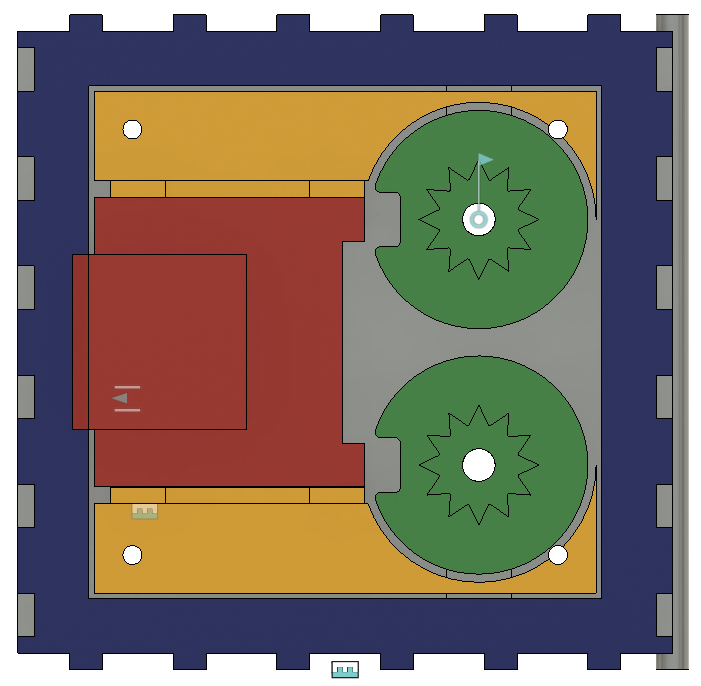
\includegraphics[width=0.4\textwidth]{kapitoly/obrazky/M1/mechanizmus.png}
    \caption{Zelená barva značí kódovací kola, červená západku, modrá pevnou část trezoru a žluté díly distanci \centering}
    \label{fig:M1-mechanizmus}
\end{wrapfigure}
První čistě mechanická varianta, označovaná jako M1, vznikla začátkem srpna 2019, brzy po první  elektronické variantě.
Měla stále poměrně klasický vzhled trezoru -- zamykatelná skříňka se dvěma  kódovacími koly, která ovládala možnost pohybu jednoduché západky.

Tato verze byla také určená jako základ pro plánovaný upgrade na další elektronickou
variantu. Na podobné vylepšení mělo stačit odstranění kódo\-va\-cích kol a přidělání elektronické části. Toto sice fungovalo obstojně, zároveň 
i~jako motivace, ale kvůli pozdější změně konceptu mechanizmu uzavírání trezoru\footnote{místo rotační západky mechanizmus bajonetu -- viz kapitola %todo
} tento nápad padl.

Tato varianta se také ukázala jako nevhodná\footnote{kvůli přílišné náročnosti na přesnost sesazení} pro stavbu s malými dětmi, 
pro které byla určena jakožto předstupeň k variantě elektronické (která vyžaduje i~znalosti programování nebo alespoň ochotu se jej  učit).

\newpage

% Zaver prace
\chapter*{Závěr}
V závěru by mělo být:
\begin{itemize}
    \item Rekapitulace cíle práce
    \item Dosáhnul jsem jej? Ano, nebo ne?
    \item Zhodnocení průběhu práce
    \item Co mi práce dala?
\end{itemize}

\newpage
\newpage

\appendix
\addcontentsline{toc}{chapter}{Přílohy}

% Prilohy
% \chapter{Obrazové přílohy}

\begin{figure}[h]
    \centering
    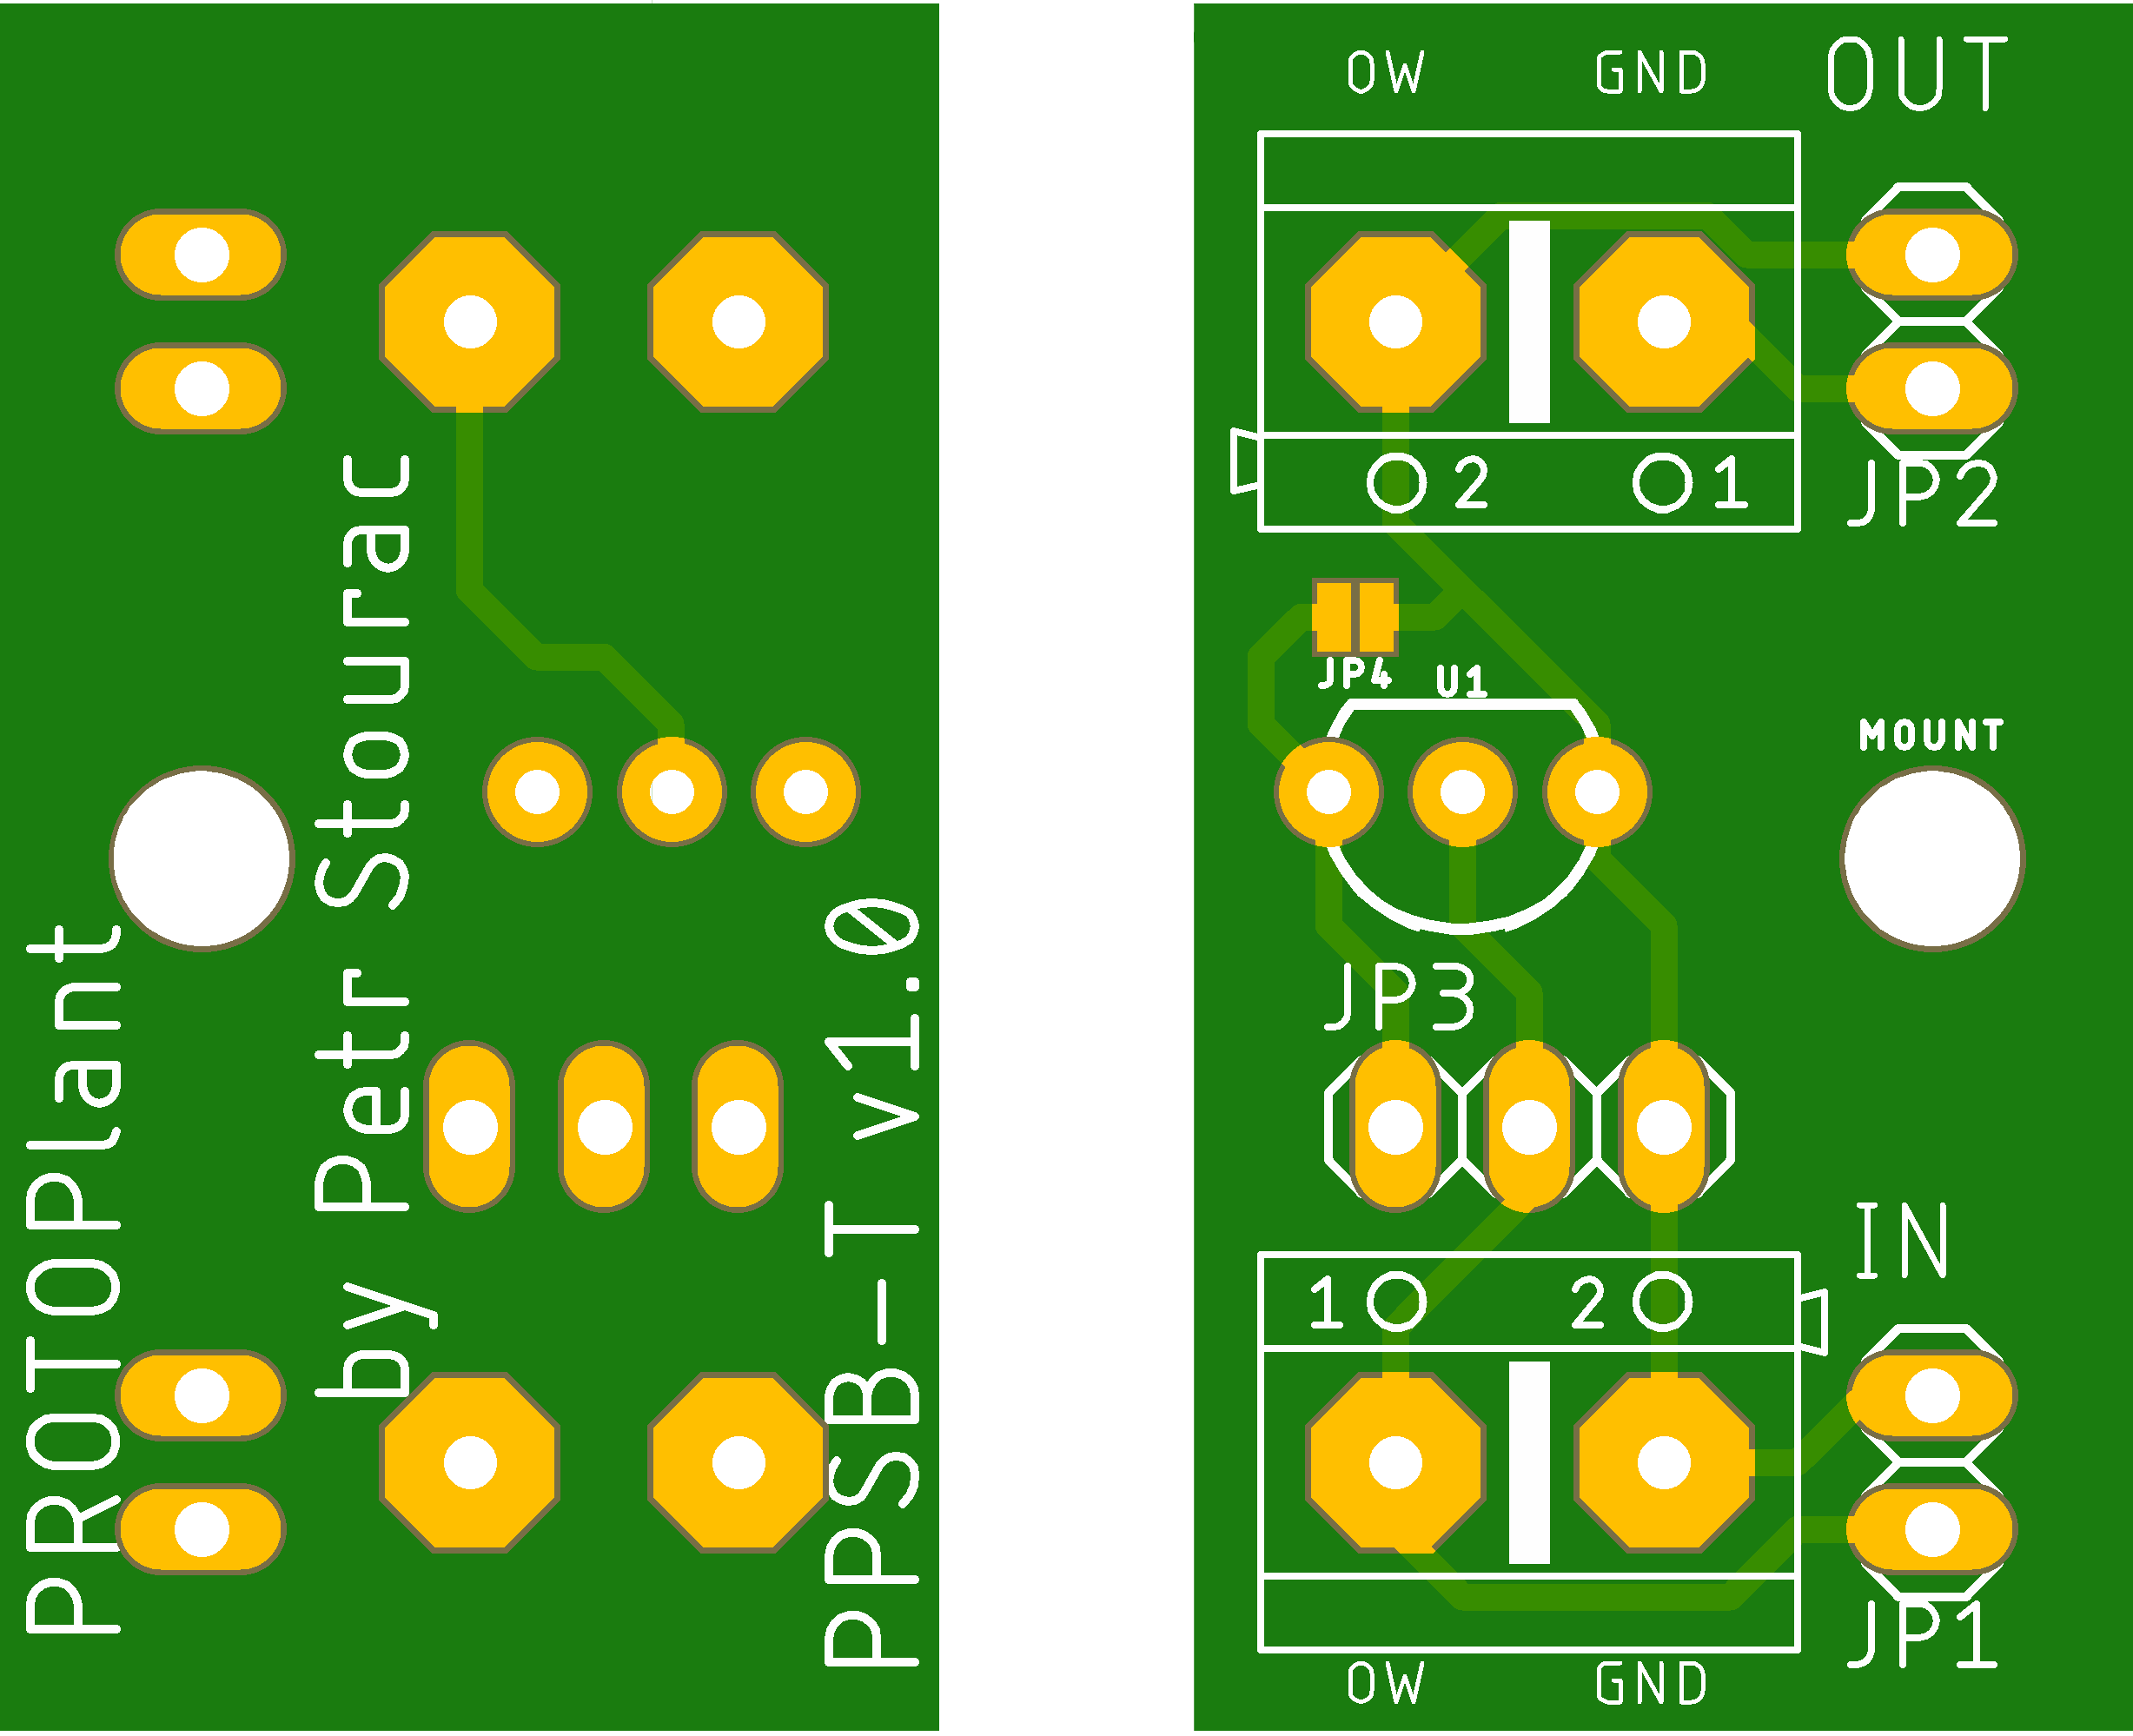
\includegraphics[width=0.85\textwidth]{img/HARDWARE/PPSB-T_BOTH.png}
    \caption{Vizualizace PPSB-T (horní strana vpravo, dolní vlevo).}
    \label{fig:PPSB-T_VISUAL}
\end{figure}

\begin{figure}[h]
    \centering
    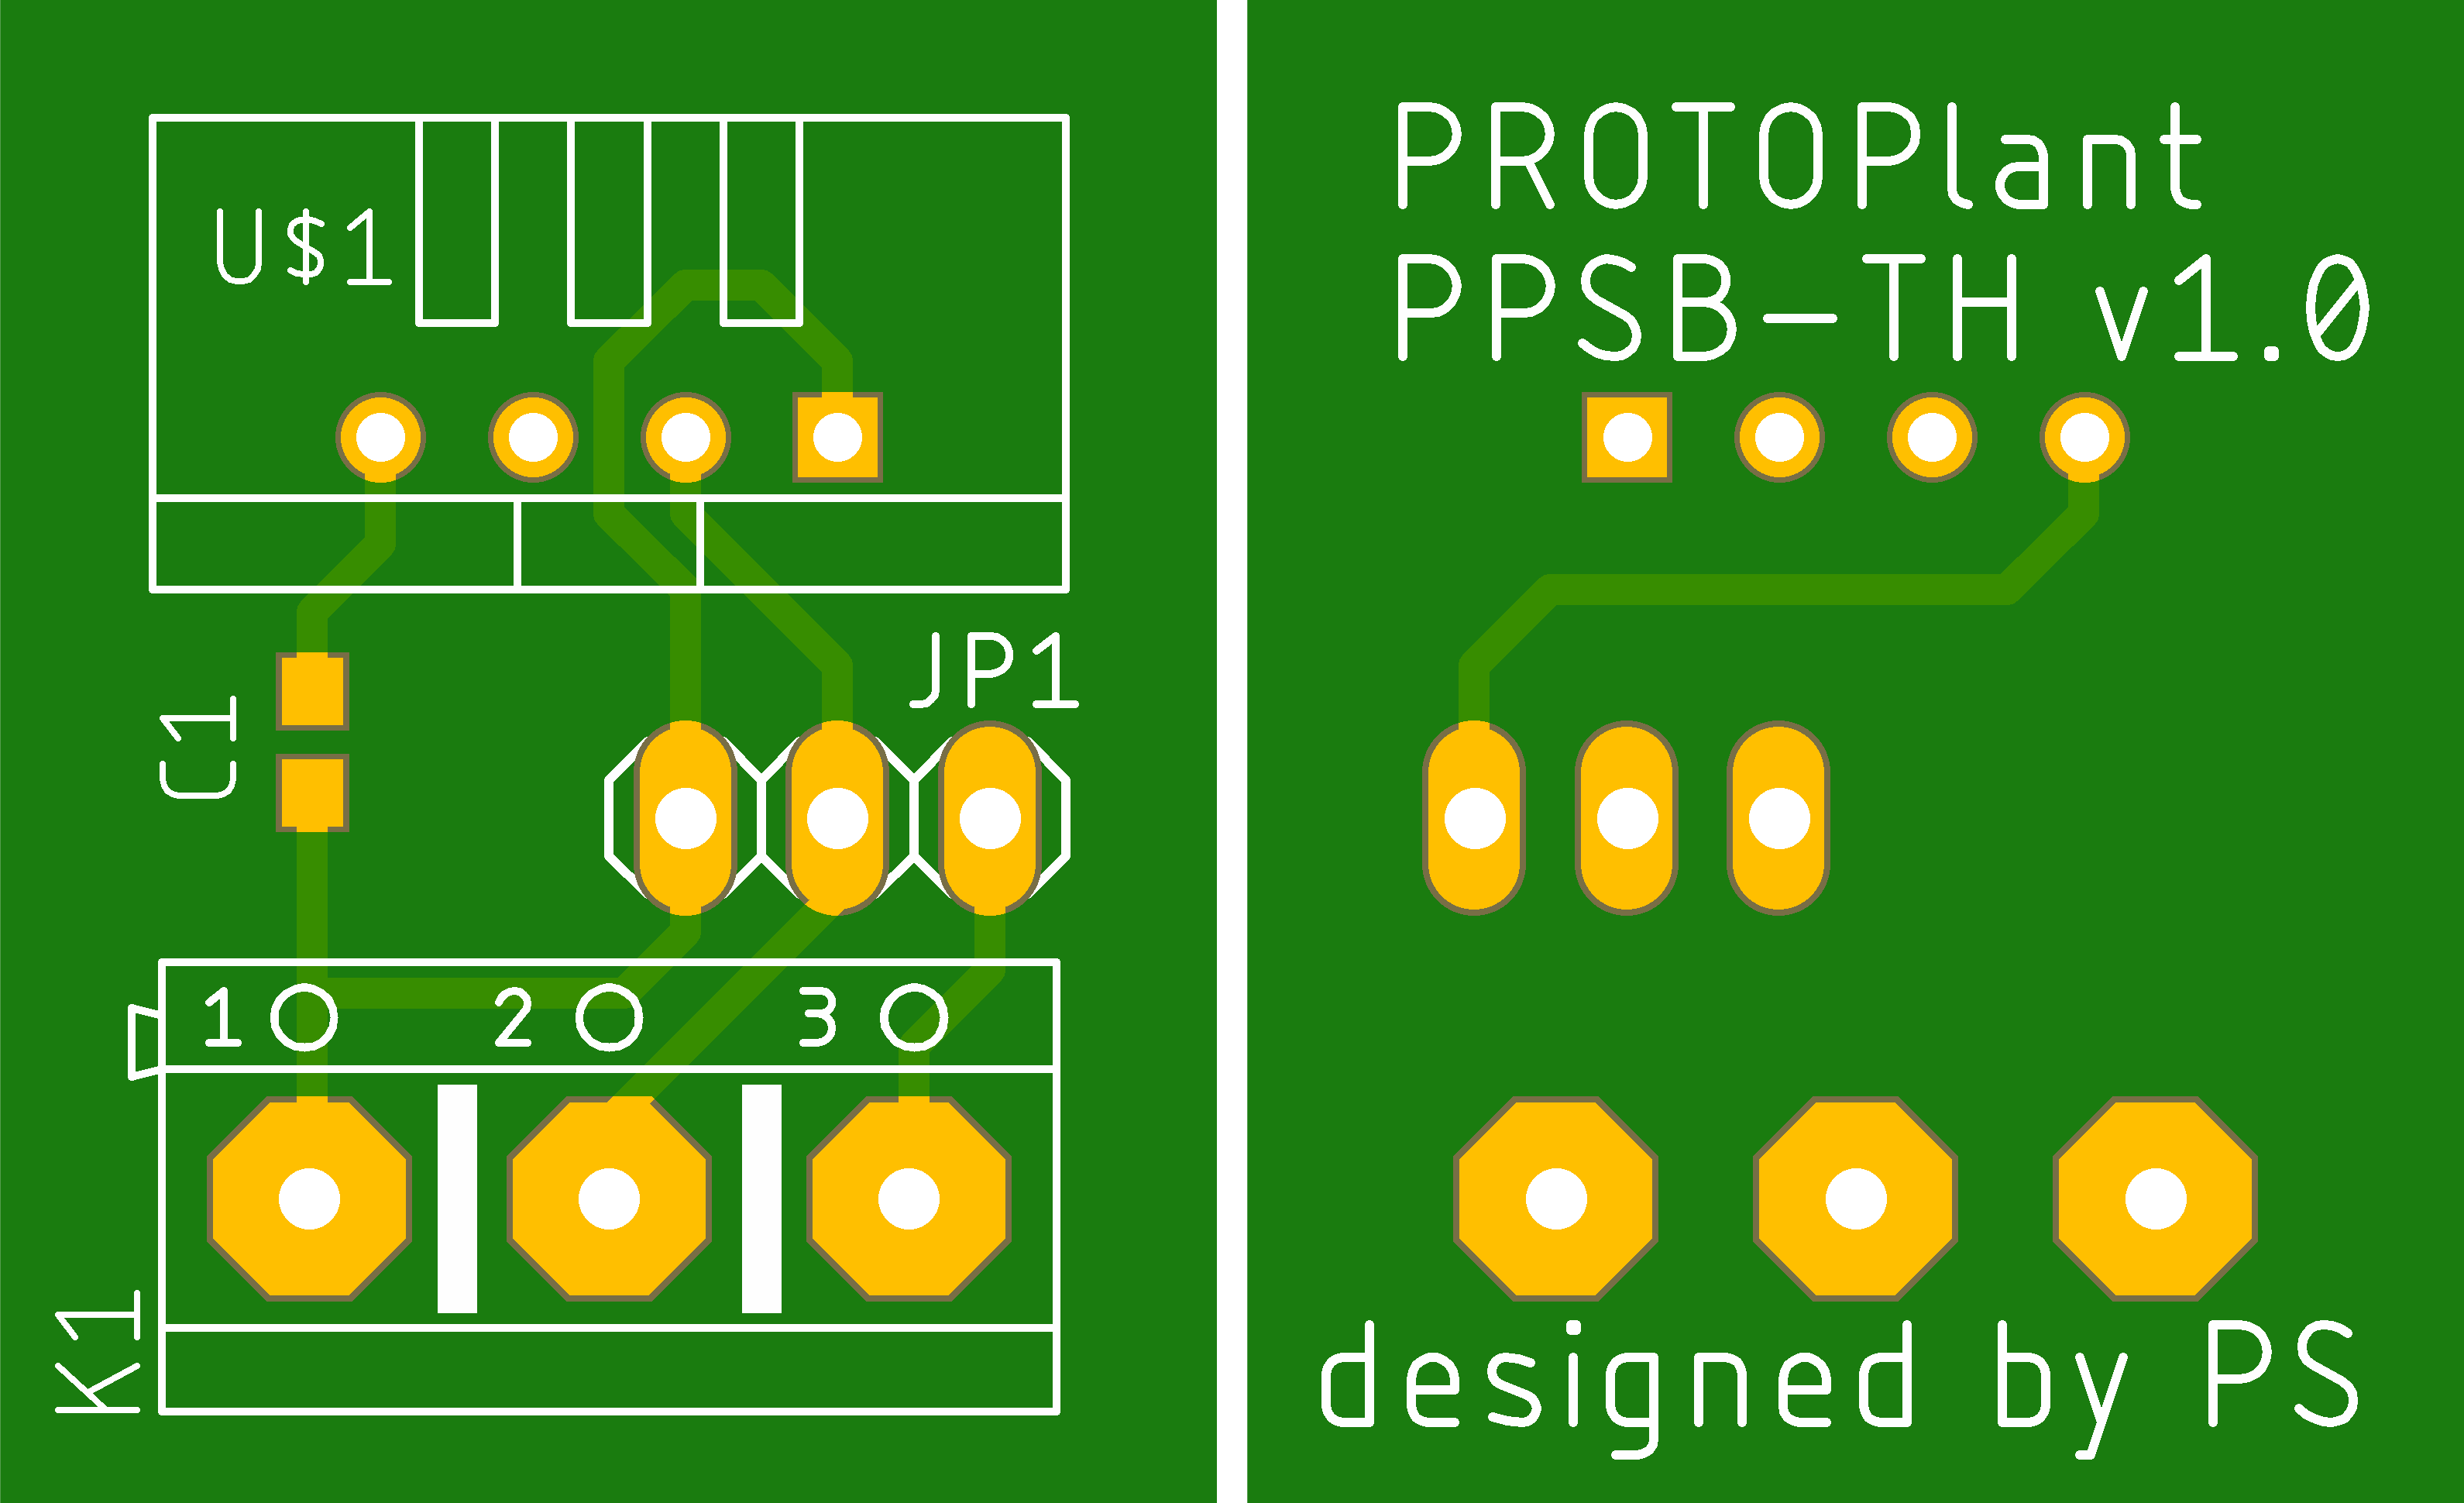
\includegraphics[width=0.85\textwidth]{img/HARDWARE/PPSB-TH_BOTH.png}
    \caption{Vizualizace desky PPSB-TH (horní strana vlevo, dolní vpravo).}
    \label{fig:PPSB-TH_VISUAL}
\end{figure}

\begin{figure}[htbp]
    \centering
    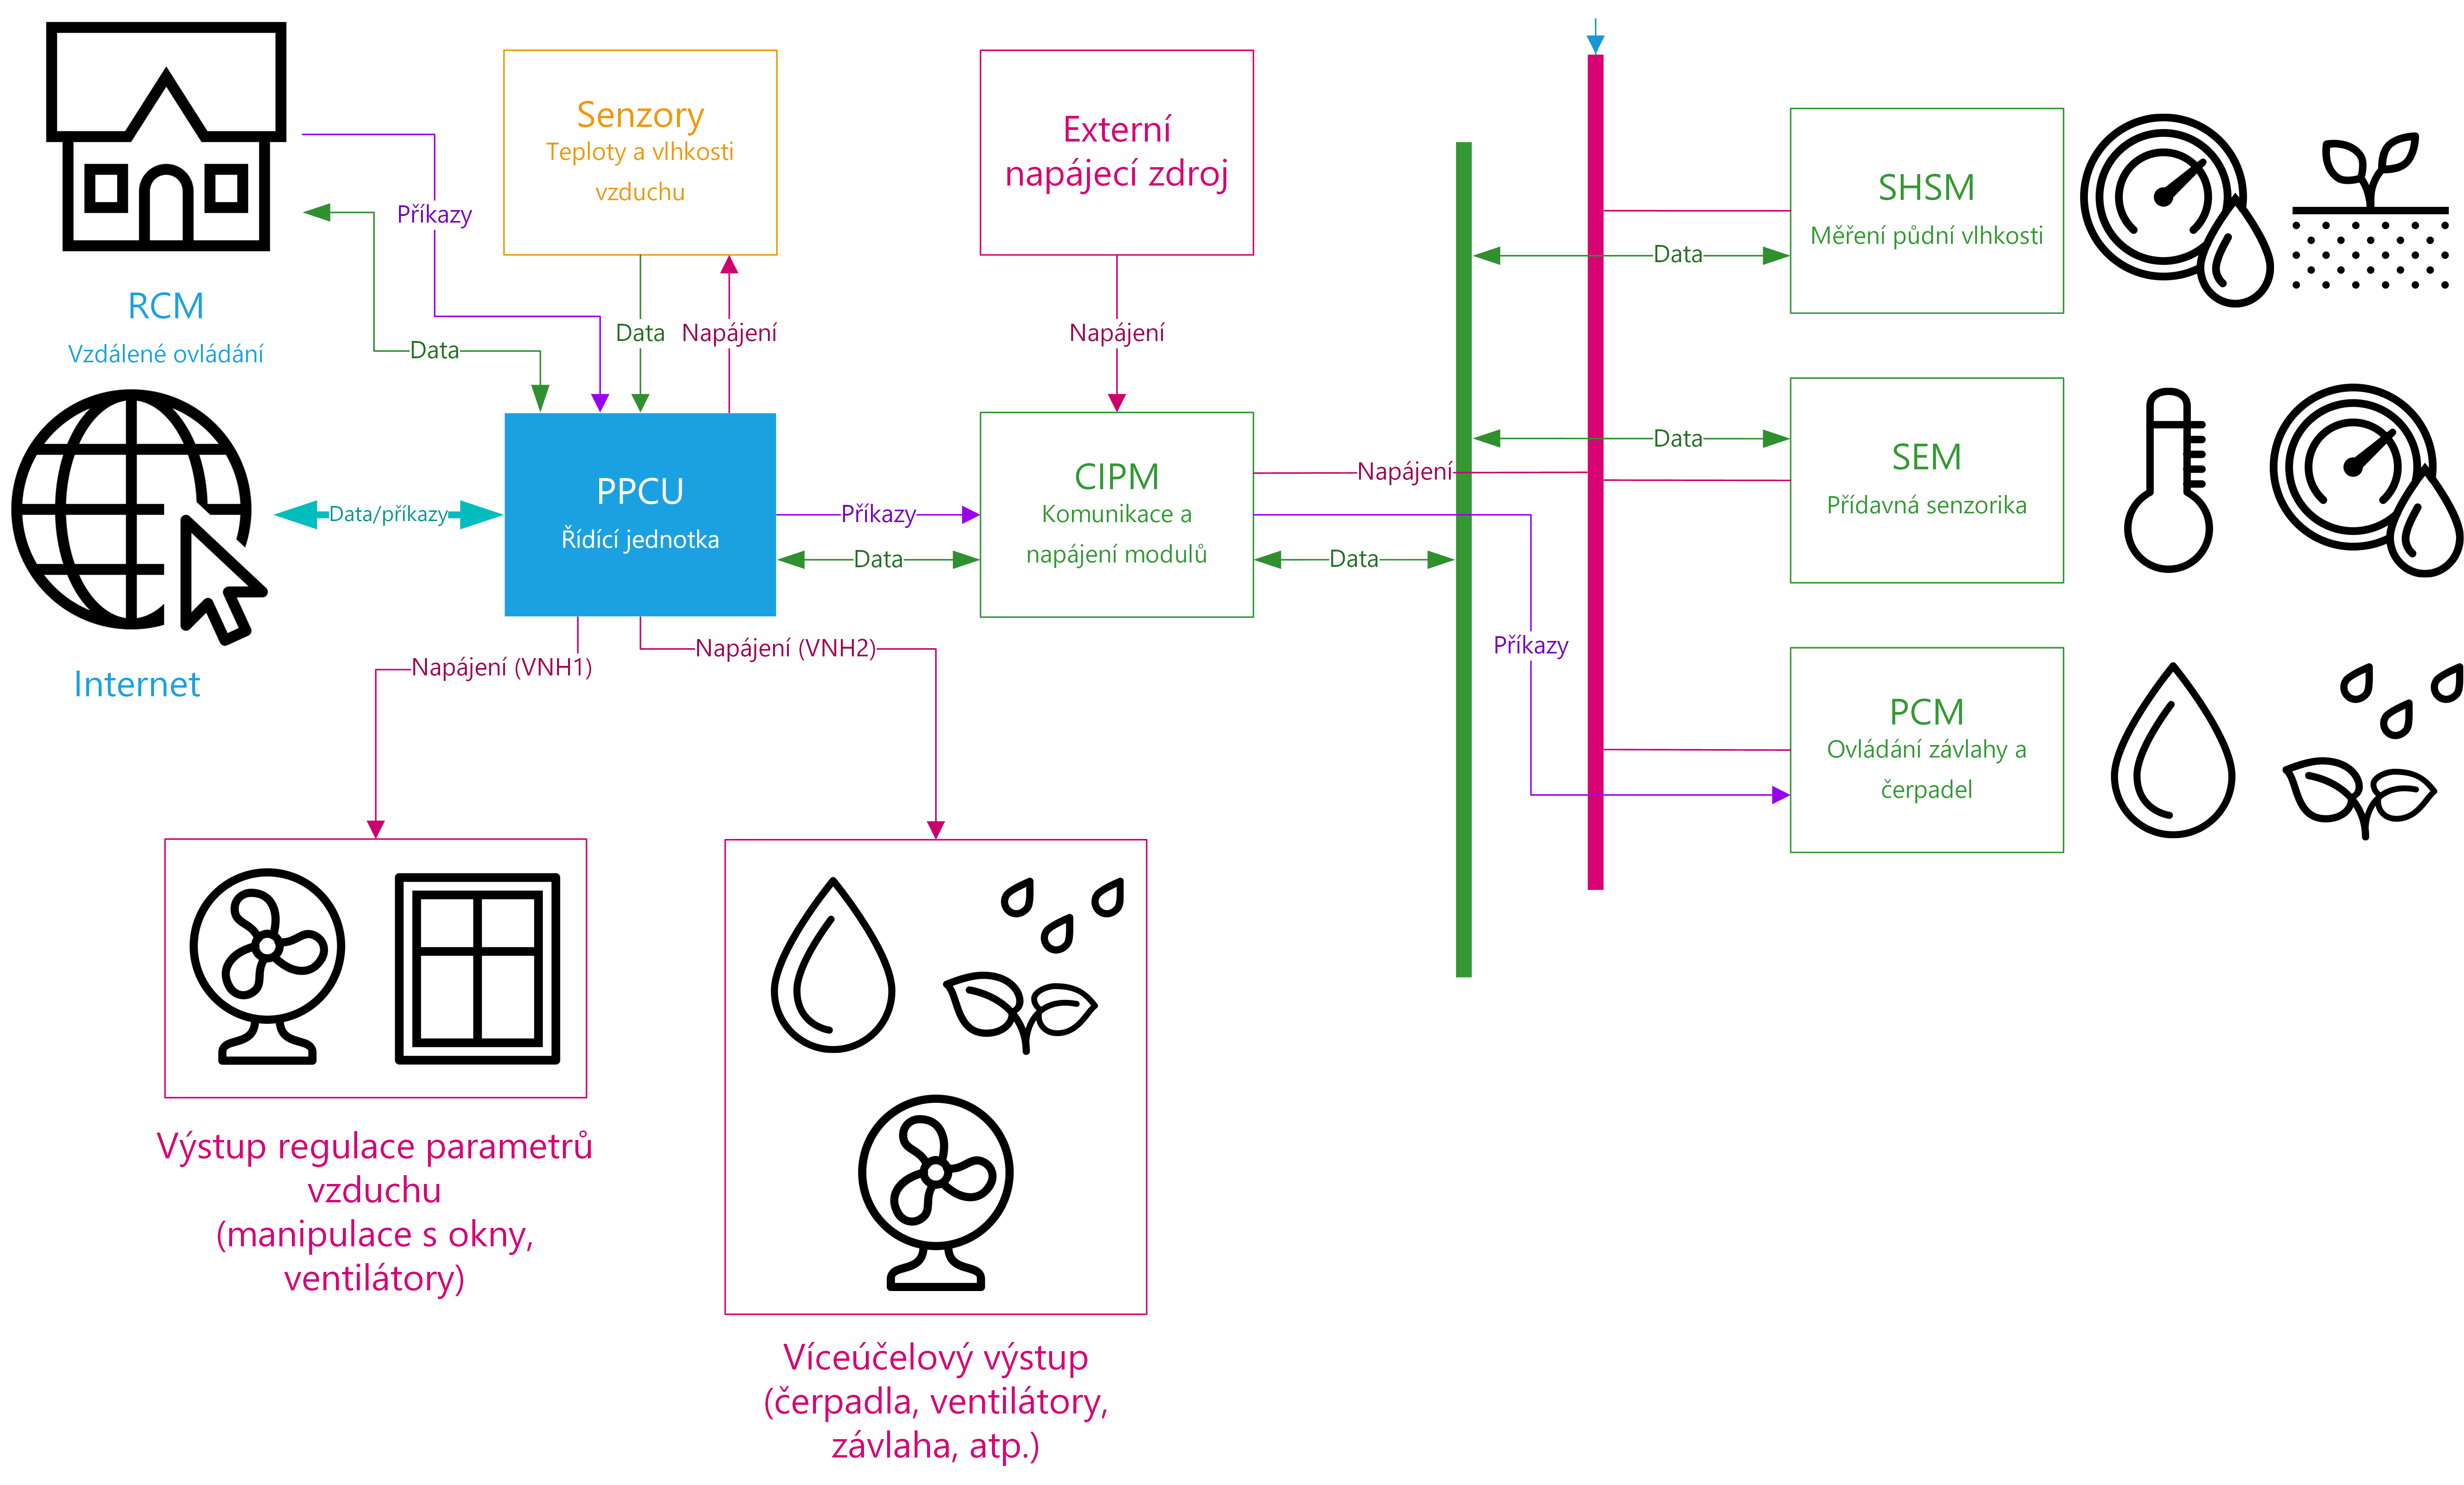
\includegraphics[angle=90,origin=c,scale=0.7]{img/HARDWARE/MODULES.png}
    \caption{Schéma zapojení a~funkce jednotlivých modulů.}
    \label{fig:add-MODULES}
 \end{figure}

\begin{figure}[h]
    \centering
    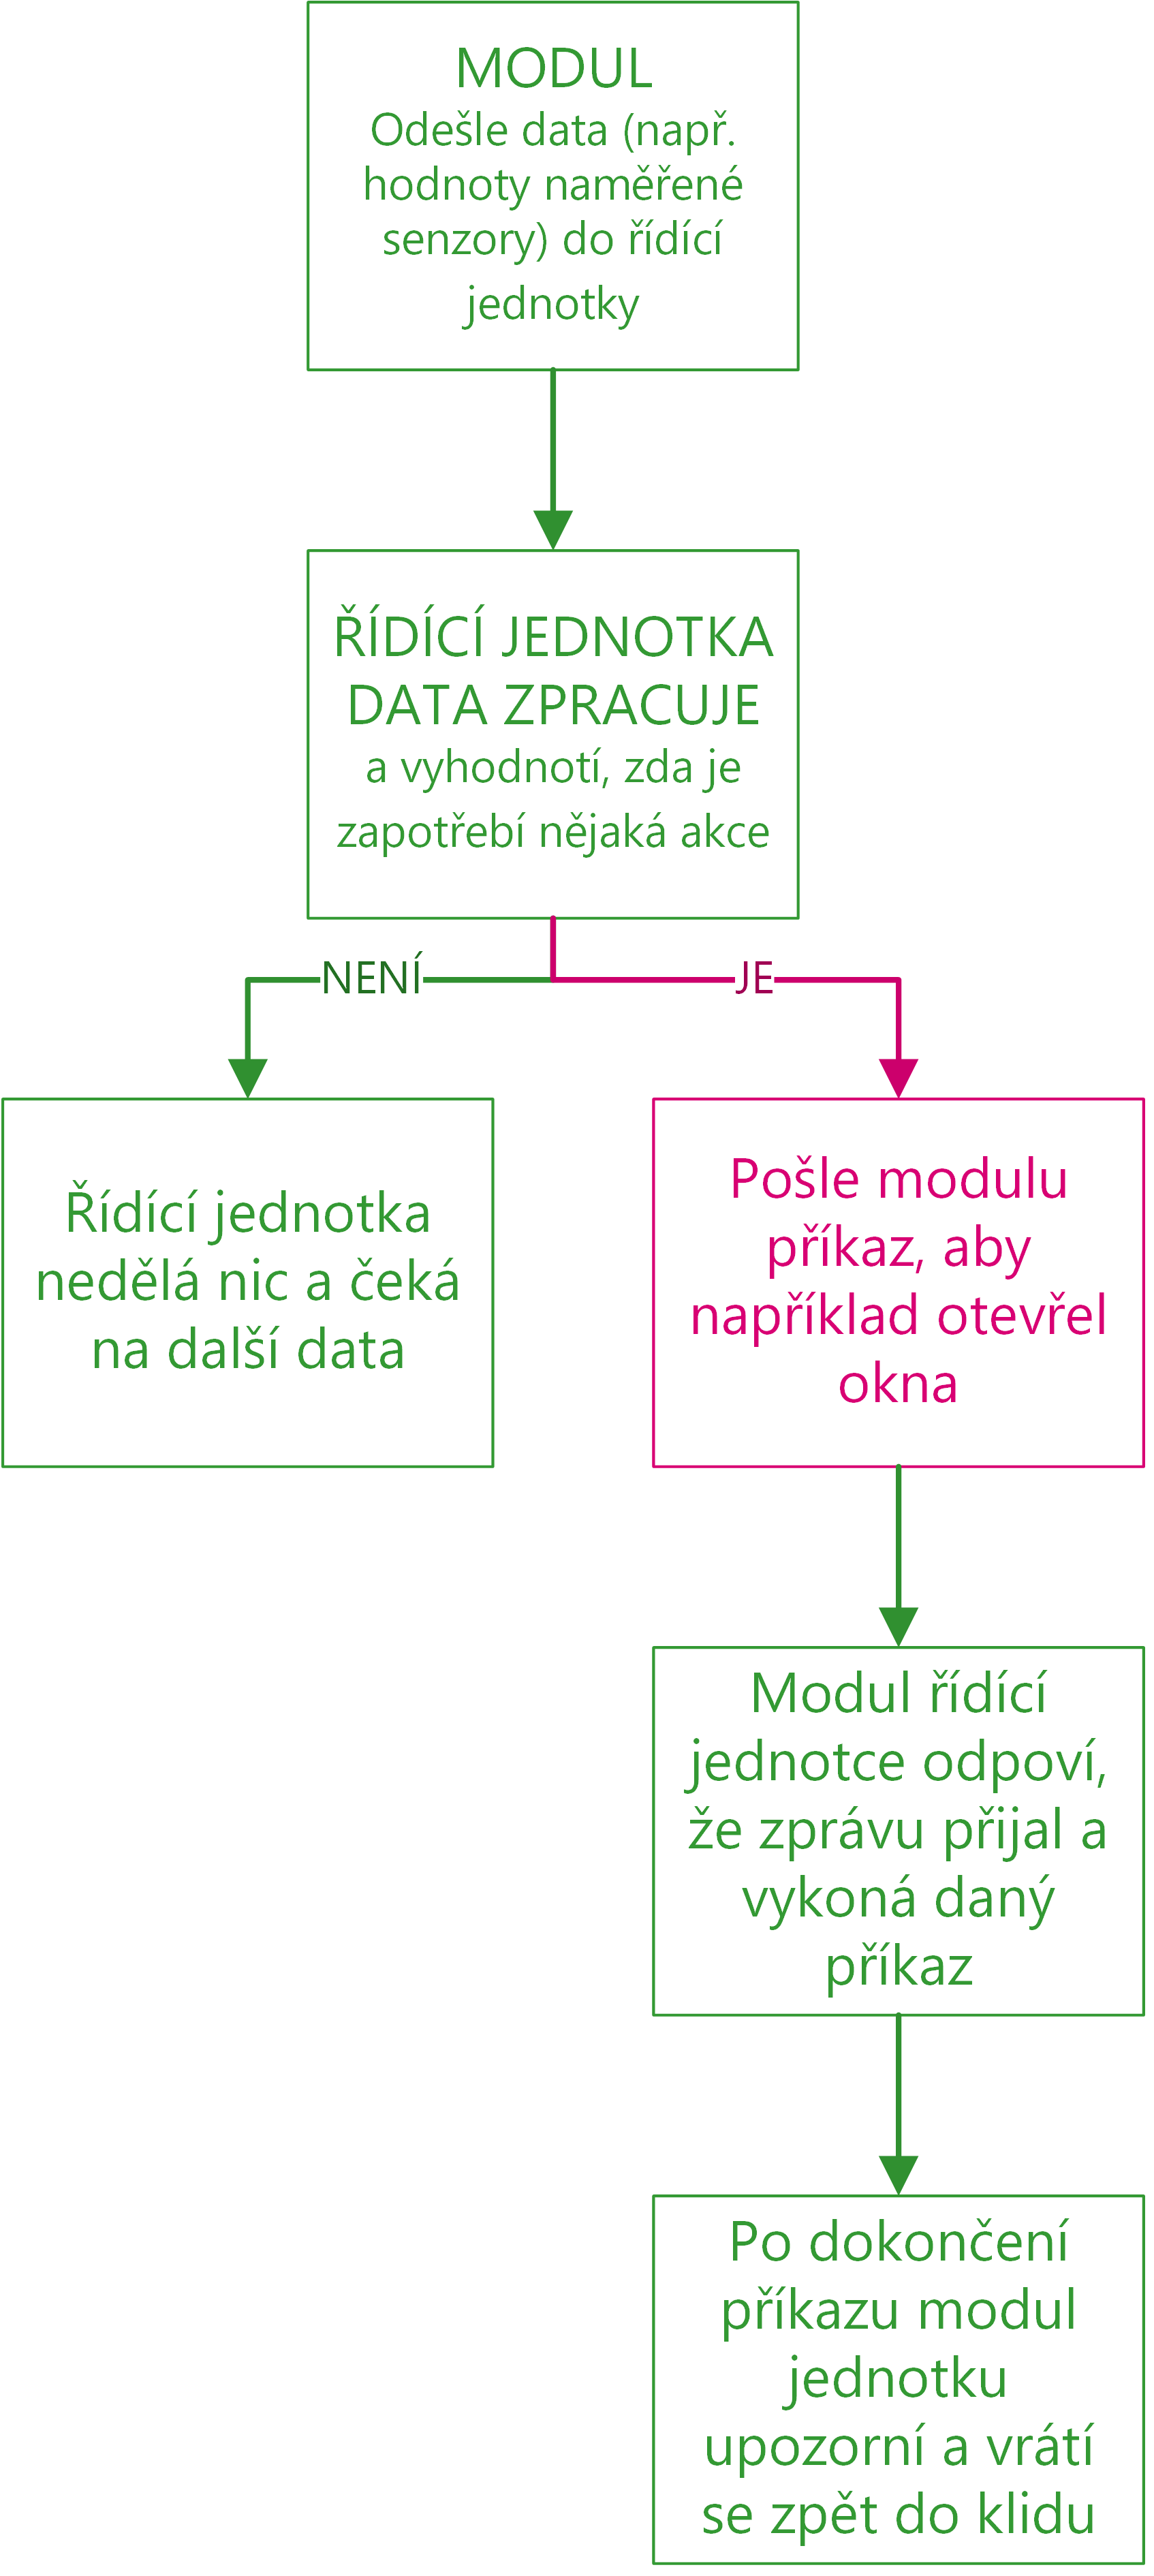
\includegraphics[scale=0.9]{img/SOFTWARE/KOMUNIKACE_MODULU.png}
    \caption{Blokový diagram komunikace řídící jednotky a~přídavného modulu.}
    \label{fig:PPCU-to-MODULE-communication}
\end{figure}

Stejným způsobem lze sázet další obrazové přílohy.
\newpage

\printbibliography[title=Literatura]
\addcontentsline{toc}{chapter}{Literatura}

\listoffigures
\addcontentsline{toc}{section}{Seznam obrázků}

\listoftables
\addcontentsline{toc}{section}{Seznam tabulek}

\end{document}
